\section{Introducción}

La \textbf{calidad del software}, tanto a nivel \textit{producto} como \textit{proceso}, 
es un aspecto muy importante dentro de la disciplina de desarrollo de software, ya que
determina el grado en que un producto satisface los requerimientos de sus usuarios, y cómo
les aporta valor.
Se considera que un \textit{modelo de calidad} tiene el objetivo de describir, evaluar y/o 
predecir la calidad de un componente \cite{Wagner2013}.
Uno de los modelos actuales, viene establecido por la familia de normas ISO/IEC 25000 \cite{ref}, 
la cual provee guías para obtener un producto de calidad, mediante la especificación 
de requisitos y características de calidad, así como la evaluación de las mismas.
Esta familia de normas está bastada en dos normas anteriores (ISO/IEC 9126 \cite{ref}
e ISO/IEC 14598 \cite{ref}), y proporcian el estándar conocido como SQuaRE 
\textit{(System and Software Requirements and Evaluation)}.

ISO/IEC 25000 presenta cinco divisiones, las cuales se enfocan en diferentes aspectos
de la calidad de software, y su proceso.
Particularmente, la norma ISO/IEC 25010, describe el modelo de calidad tanto para el producto
y uso; definiendo así las características y subcaracterísticas utilizadas en la evaluación
de un elemento.
Este modelo determina ocho características, junto con sus subcaracterísticas, y éstas son:
\begin{itemize}
    \item Adecuación funcional
    \item Eficiencia de desempeño
    \item Compatibilidad
    \item Usabilidad
    \item Fiabilidad
    \item Seguridad
    \item Mantenibilidad
    \item Portabilidad
\end{itemize}

La que mayor interés suscinta para el presente informe, corresponde a la característica
de \textbf{Mantenibilidad}, la cual representa la \textit{capacidad del software para ser modificado
de forma eficiente y efectiva, ya sea por motivos correctivos, evolutivos o perfectivos}.
Ésta, se compone así mismo de cinco subcaracterísticas, las cuales son descritas
a continuación:
\begin{description}
    \item [Modularidad] Corresponde al grado de descomposición de un programa en otros más pequeños
    con interfaces estandarizadas, y la capacidad de permitir que un cambio en un componente tenga
    un impacto mínimo en los demás.
    \item [Reusabilidad] Determina la capacidad de que un activo o elemento sea empleado en más
    de un sistema de software, o en la construcción de otros elementos.
    \item [Analizabilidad] Asociada a la facilidad con la que se puede identificar las partes
    a modificar y la evaluación del impacto generado por el cambio, así como también el diagnóstico
    de problemas o causas de fallas en el software.
    \item [Capacidad para ser modificado] Es la capacidad del producto para ser modificado de
    forma efectiva y eficiente, sin introducir defectos o afectar la performance.
    \item [Capacidad para ser probado] Corresponde a la facilidad con la que se pueden definir
    parámetros de prueba de un sistema/componente, y la posibilidad de ejecución de dichas pruebas,
    para determinar si se cumplen los criterios establecidos.
\end{description}

Así como la familia de normas ISO/IEC 25000 define un conjunto de características y
subcaracterísticas, también provee un listado básico de métricas para efectuar la
medición de las las nombradas previamente.
Este listado no es exhaustivo, ya que se pueden utilizar métricas no definidas por el
estándar, siempre y cuando se determine su correlación con alguna de las características
establecidas.
En la tabla \ref{Metrics} se listan las métricas definidas por el estándar, para la \textit{Mantenibilidad}
y sus subcaracterísticas.

\begin{figure}[H]
    \label{Metrics}
    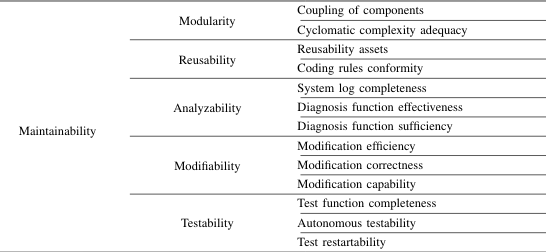
\includegraphics[width=12cm]{quality_metrics/quality_metrics.png}
    \centering
    \caption{Métricas para Mantenibilidad y su subcaracterísticas}
\end{figure}

En el contexto de este trabajo, las subcaracterísticas de mayor interés corresponden
a la \textbf{analizabilidad} y la \textbf{capacidad de ser modificado}, también llamada
\textit{modificabilidad}.

Desde el punto de vista de la \textbf{analizabilidad}, se definen tres métricas.
La \textit{Completitud de Logs del Sistema} se refiere a la proporción de logs que son
efectivamente registrados en un sistema.
La \textit{Efectividad de las Funciones de Diagnóstico} y \textit{Suficiencia de las
Funciones de Diagnóstico} miden la proporción de funciones de diagnóstico implementadas que
son realmente útiles, y la proporción de funciones de diagnóstico requeridas que están
implementadas, respectivamente.

Con respecto a la \textbf{modificabilidad}, la \textit{Eficiencia de Modificación} se mide
como el tiempo promedio que lleva un cambio, normalizado con respecto al tiempo esperado
para el mismo.
La \textit{Correctitud de Modificación} midel la proporción de cambios que no causan un
degradamiento en la calidad del sistema; mientras que la \textit{Capacidad de Modificación}
corresponde a una proporción de cambios que pueden ser implementados en un período determinado
de tiempo.

Todas estas métricas tratan de ayudar a determinar cuál es el nivel de calidad correspondiente a
un sistema o componente de software, de acuerdo a las características antes mencionadas.
Sin embargo, este conjunto de normas como otras existentes o anteriores sólo ofrecen una
guía muy abstracta sobre la definición de calidad de software, y no indican cómo lograr
que el software sea de calidad \cite{Relf04}.

"ISO-9126 defines a set of six quality attributes: efficiency, functionality, maintanability,
portability, realiability and usability.
However, standards like ISO-9126 only offer top-level guidance that define software quality,
they do not prescribe how to insert quality into software (Dromey, 1995).
Some objective measure of software quality is required in order to categorise acceptable
practices (Vollman, 1993) and software quality will not improve until there is a comprehensive
definition available"\cite{Relf04}.

\section{Modelos de Calidad -Historia y falencias}

La investigación relacionada a la calidad de software, viene desde casi tanto tiempo como
la investigación del software en sí misma.
A lo largo de las últimas cuatro décadas, se han ido proponiendo diferentes y diversos 
modelos \cite{Deissenboeck2009}.
Dentro de los primeros modelos, escritos a finales de la década de 1970, aparecen los
propuestos por Boehm et al. \cite{Boehm1978} y McCall et al. \cite{McCall1977}, los cuales trataban
de definir la calidad de software como una descomposición jerárquica de características y
subcaracterísticas.
Si bien proveyeron definiciones sólidas sobre los diferentes aspectos de la calidad de software,
no propusieron una forma de, confiablemente, evaluar las características tanto individualmente
o como un todo.
Por lo tanto, la investigación subsiguiente se enfocó principalmente en encontrar maneras de
cuantificar las propiedas definidas por los estudios anteriores.
Los trabajos de Dromey \cite{Dromey1995} y de Bansiya y Davis \cite{Bansiya2002}, son los más 
importantes ya que forman la base sobre la cual se construyeron los modelos más recientes, al 
describir cómo los atributos de alto nivel de calidad pueden medirse a partir de \textit{propiedades
de bajo nivel}, cuantificadas desde métricas de software y análisis estático.

Las contribuciones más significativas en el campo de la \textit{evaluación cuantitativa de la calidad},
basadas en el \textbf{análisis estático de código fuente} vienen dadas por el Modelo de Mantenibilidad 
SIG \cite{Heitlager2007}, junto con Quamoco tool chain \cite{Wagner2012}.

\subsection{Modelo de Mantenibilidad SIG}

Este modelo de evaluación de calidad \cite{Heitlager2007} permite determinar la mantenibilidad
de un proyecto de software.
Las características de mantenibilidad son descompuestas en un conjunto de subcaracterísticas,
y estas últimas en \textit{propiedades}.
Estas propiedades son cuantificables directamente desde el código fuente del producto, utilizando
análisis estático, y a partir de estos valores junto con unos determinados umbrales,
cada propiedad recibe un \textit{perfil de calidad}.
Al poder cuantificar estas propiedades y obtener los perfiles, también se pueden agregar
para así establecer un puntaje global de calidad del sistema.
Los umbrales empleados en la evaluación de los propiedades son obtenidos a través de
benchmarking, con el fin de mantener la objetividad \cite{Alves2010}.

\subsection{Quamoco Tool Chain}

Similar al Modelo de Mantenibilidad SIG \cite{Heitlager2007}, Quamoco Tool Chain \cite{Wagner2012}
se basa en propiedades extraídas desde el código fuente a través de análisis estático del mismo,
con la diferencia de que permite a los interesados definir sus propios modelos jerárquicos
de calidad.
Quamoco define un meta-modelo, facilitando la creación de modelos más genéricos, en lugar de
estar restringidos a ciertos atributos de calidad, como lo es la mantenibilidad.

The meta model introduces the new concept of a product factor, which bridges the gap between
concrete measurements and abstract quality aspects.
Product factors have measures and instruments to operationalise quality by measurements from
manual inspection and tool analysis.
The base model uses the ISO 25010 quality attributes, which we refine by 200 factors and 600
measures for Java and C Sharp systems.

\subsection{Low-level metrics}

\section{Impacto de los identificadores en Calidad de Software}

"The impact of low quality identifier names on program comprehension is reasonably
well understood \cite{DeiBenbockPizka05,Lawrie2007,Lawrie2006}, but little is known
about the extent to which the quality of identifier names might influence the quality
of source code" \cite{ButlerWemelingerYu10}.

"Buse and Weimer \cite{Buse2008} developed a readability metric for Java derived from measurements 
of, among others, the number of parentheses and braces, line length, the number
of blank lines, and the number, frequency and length of identifiers.
Using machine learning, the readability metric was trained to agree with the judgement 
of human source code readers.
Buse and Weimer found a significant statistical relationship between the readability of 
methods and the presence of defects found by FindBugs in open source code bases. 
Although their work makes a link between readability and software quality, their notion
of readability ignores the quality of identifier names".

Se ignora el contenido semántico.

"The predictive probability associated with each relationship illustrates the utility
of the identifier flaws as light-weight classifiers for source code quality"
\cite{ButlerWemelingerYu10}.

\textbf{"a low-cost heuristic to identify potentially problematic regions of source code"}

"Software quality is not defined in terms of quality attributes but instead must be
inferred from characteristics that correlate to quality attributes and defect attributes.
One of these quality attributes is the readability of the software.
However, the software engineer, who is ultimately responsible for software quality,
is not supported well by their formal education, the software engineering culture, the
existence of useful tools and where these tools do exist by their limited up-take by industry.
Human cognitive limitations similarly frustrate the development of readable source code.
Software characteristics have been identified, which correlate well to source code readability.
One of these software characteristics, which have been supported by empirical research,
is the choice of identifier name".\cite{Relf04}

"A software characteristic that has the potential to improve software quality is the choice of
identifier name, and this is particularly so in large software systems.
identifier-naming sytle guidelines, supported by empirical evidence and generally accepted by
software professionals to direct towards improved source code readabiity are candidates for
automation by a tool.
Such an automated tool could make visibile aspects of software quality that are less keenly
perceived by the novice programmer and could assist in ther education along the path to
expert status"\cite{Relf04}.

"Existing research on source code readability focuses on the contribution the
components of source code make to readability" \cite{Buse2008}.

\textit{A partir de acá, métricas.
Posibilidad de usar elementos de (measurement, measure, metric, etc) para la definición de
la métrica puntual.}
